\documentclass{article}
\usepackage[utf8]{inputenc}
\usepackage{amsmath, amssymb, amsthm}
\usepackage{graphicx}
\usepackage{witharrows}

\title{PWM Simulation and Characterization}
\author{Kadyn Belesca}
\date{1/28/2024}

\begin{document}

\maketitle

\newpage

\section{PWM Defined as a Function of Duty Cycle}

We can define a PWM signal with amplitudes of -1 to 1 as a function of duty cycle like so:

\begin{equation}
x(t) =
    \begin{cases}
    1 & 0 \leq t \leq \alpha{T_{0}} \\
    -1 & \alpha{T_{0}} \leq t \leq T_{0}(1 - \alpha) \\ 
    \end{cases}
\end{equation}

Where:

\vspace{5mm}

$T_{0} =$ Fundamental Period

$\alpha =$ Duty Cycle

\subsection{PWM Example}
Figure 1 is an example of a PWM square wave signal at 179 kHz, which is my student ID number rounded up to 3 significant digits,
at 25 percent duty cycle. For the following calculations, we will use this example at different duty cycles.
\begin{figure}[h]
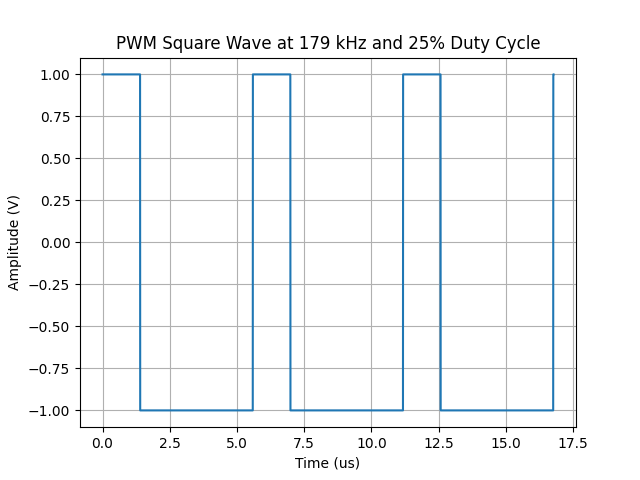
\includegraphics[scale=.70]{squarewave.png}
\caption{PWM Example}
\end{figure}

\newpage

\subsection{Derivation of Frequency Spectra}

We can derive the math defintion using a Fourier Transform to get the signal in the frequency spectra.
Since this is a PWM square wave, we will need to setup an improper integral defining the amplitudes at
their specified time intervals. 

\begin{gather*}
\int_a^b \! x(t)e^{-j\omega{t}} \, \mathrm{d}t = \int_{a_1}^{b_1} \! 1e^{-j\omega{t}} \, \mathrm{d}t + \int_{a_2}^{b_2} \! -1e^{-j\omega{t}} \, \mathrm{d}t \\
= \int_{a_1}^{b_1} \! e^{-j\omega{t}} \, \mathrm{d}t - \int_{a_2}^{b_2} \! e^{-j\omega{t}} \, \mathrm{d}t \\
\text{We can pull out $\frac{1}{\omega{j}}$ from the resulting Riemann sums.} \\
= \frac{1}{\omega{j}}[[-e^{-\omega{jb_{1}}}+e^{-\omega{ja_{1}}}]+[e^{-\omega{jb_{2}}}+e^{-\omega{ja_{2}}}]] \\
\text{Then we can combine both Riemann sums into one whole} \\
\text{Riemann sum and use Euler's formula on the terms.} \\
= \frac{1}{\omega{j}}(-\cos{\omega{b_1}}-j\sin{\omega{b_1}}+\cos{\omega{a_1}}+j\sin{\omega{a_1}}+\cos{\omega{b_2}}+j\sin{\omega{b_2}}+\cos{\omega{a_2}}+j\sin{\omega{a_2}}) \\
\text{Since $b_1=a_2$ and $a_1=0$, we can cancel out some terms.} \\
= \frac{1}{\omega{j}}(1+\cos{\omega{b_2}}+j\sin{\omega{b_2}}) \\
\text{Using the following (adjusted) Euler's identity we can derive the complete Fourier transform.} \\
\sin{\omega} = \frac{1}{2j}(\cos{\omega}+j\sin{\omega}-\cos{\omega}+j\sin{\omega}) \\
\text{We can balance out the above equation with our equation we got in the previous integration.} \\
\sin{\omega{b_2}} = \frac{1}{2j}(\cos{\omega{b_2}}+j\sin{\omega{b_2}}-\cos{\omega{b_2}}+j\sin{\omega{b_2}}) \\
\text{First is to balance the $\frac{1}{2j}$ coefficient with the our coefficient} \\
\frac{2\sin{\omega{b_2}}}{\omega} = \frac{1}{\omega{j}}(\cos{\omega{b_2}}+j\sin{\omega{b_2}}-\cos{\omega{b_2}}+j\sin{\omega{b_2}}) \\
\text{Next, we expand the term on the right and add $\frac{1}{\omega{j}}$} \\
\frac{2\sin{\omega{b_2}}}{\omega}+\frac{1}{\omega{j}} = \frac{1}{\omega{j}} + \frac{\cos{\omega{b_2}}}{\omega{j}}+\frac{j\sin{\omega{b_2}}}{\omega{j}}-\frac{\cos{\omega{b_2}}}{\omega{j}}-\frac{j\sin{\omega{b_2}}}{\omega{j}} \\
\text{We can then add $\frac{\cos{\omega{b_2}}}{\omega{j}}+\frac{j\sin{\omega{b_2}}}{\omega{j}}$ to both sides,} \\
\text{cancel out some $j$'s, and combine like-terms to get the resulting Fourier transform:} \\
X(t) = \frac{3\sin{\omega{b_2}}}{\omega}-j\frac{1+\cos{\omega{b_2}}}{\omega} \\
\end{gather*}

\subsection{Further Calculations and Explainations}

From our equation $X(t) = \frac{3\sin{\omega{b_2}}}{\omega}-j\frac{1+\cos{\omega{b_2}}}{\omega}$, we can understand a few things.
First, since $b_2 = T_0(1-\alpha)$, we can directly get the frequency value for each point by using the equation $\frac{1}{T}$, which is the equation
for converting time to frequency. Since $b_2$ is a point in time from $0$ to $T_0$, we can replace $T$ with $b_2$ to get the resulting equation $\frac{1}{b_2}$ to get our x-values in the frequency domain.

\vspace{5mm}

For magnitude: $||\vec{X}(t)|| = \sqrt{{(\frac{3\sin{\omega{b_2}}}{\omega})}^2+{(\frac{1+\cos{\omega{b_2}}}{\omega})}^2}$

\vspace{5mm}

For phase: $\theta = \tan^{-1}{\frac{\frac{1+\cos{\omega{b_2}}}{\omega}}{\frac{3\sin{\omega{b_2}}}{\omega}}}$

\begin{figure}[h]
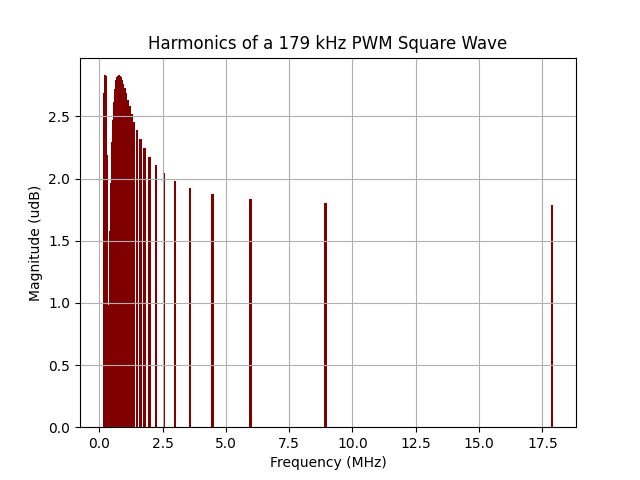
\includegraphics[scale=.70]{harmonics.png}
\caption{Harmonics of the PWM Square Wave}
\end{figure}

\begin{figure}[h]
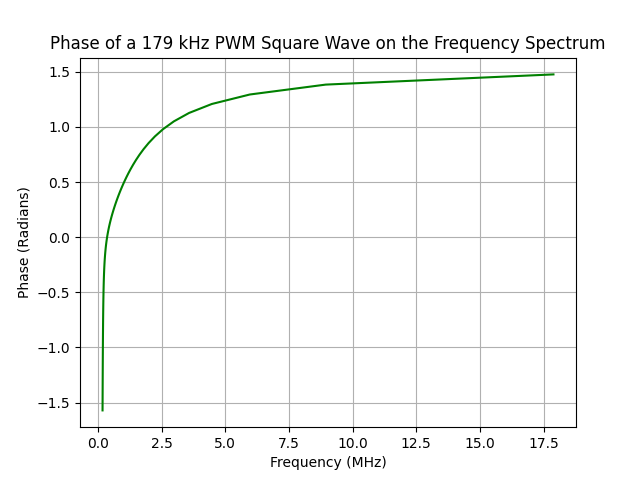
\includegraphics[scale=.70]{phase.png}
\caption{Phase of the PWM Square Wave}
\end{figure}

\begin{figure}[h]
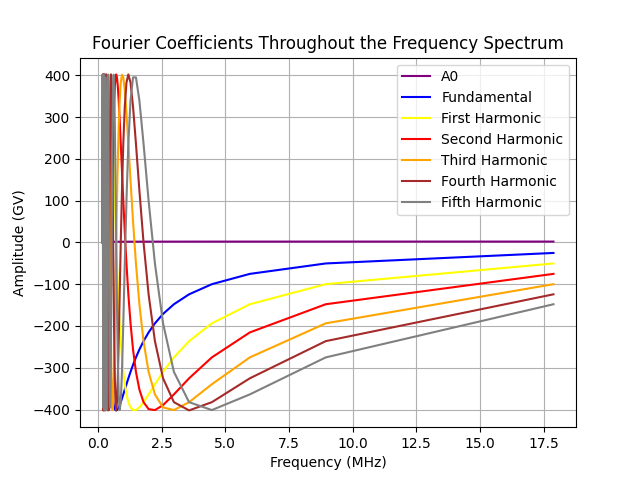
\includegraphics[scale=.70]{coefficients.png}
\caption{Coefficients Throughout the Frequency Spectrum}
\end{figure}

\end{document}